\documentclass{article}
\usepackage{tikz}
\usepackage{graphicx}

\definecolor{darkblue}{HTML}{3535B4}
\definecolor{LightSkyBlue}{HTML}{87CFFA}
\definecolor{DeepSkyBlue}{HTML}{00BFFF}
\definecolor{Greeen}{HTML}{439236}
\definecolor{mauve}{HTML}{874ad3}
\definecolor{vert}{HTML}{0ab351}
\definecolor{darkred}{HTML}{a31623}

\begin{document}

\begin{figure}[h!]
\begin{center}
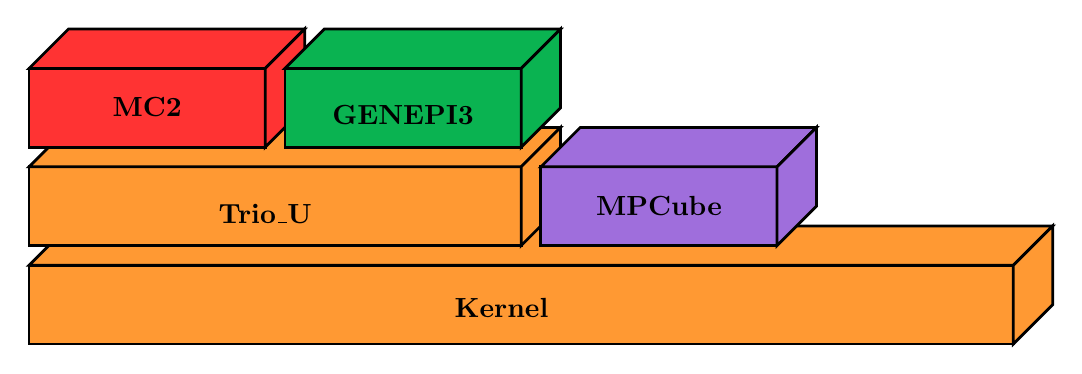
\begin{tikzpicture}[scale=2, line width=1pt]
% box Kernel
\coordinate (A) at (0,0) ;
\coordinate (B) at (6.25,0) ;
\coordinate (C) at (6.25,0.5) ;
\coordinate (D) at (0,0.5) ;
\coordinate (E) at (0.25,0.75) ;
\coordinate (F) at (6.5,0.75) ;
\coordinate (G) at (6.5,0.25) ;
\draw[black,fill=orange!80] (A) -- (B) -- (C) -- (D) -- cycle ;
\draw[black,fill=orange!80] (D) -- (C) -- (F) -- (E) -- cycle ;
\draw[black,fill=orange!80] (B) -- (C) -- (F) -- (G) -- cycle ;
\draw (3,0.1) node[above]{\textbf{Kernel}} ;
%% box Trio_U
\begin{scope}
\coordinate (A1) at (0,0.625) ;
\coordinate (B1) at (3.125,0.625) ;
\coordinate (C1) at (3.125,1.125) ;
\coordinate (D1) at (0,1.125) ;
\coordinate (E1) at (0.25,1.375) ;
\coordinate (F1) at (3.375,1.375) ;
\coordinate (G1) at (3.375,0.875) ;
\draw[black,fill=orange!80] (A1) -- (B1) -- (C1) -- (D1) -- cycle ;
\draw[black,fill=orange!80] (D1) -- (C1) -- (F1) -- (E1) -- cycle ;
\draw[black,fill=orange!80] (B1) -- (C1) -- (F1) -- (G1) -- cycle ;
\draw (1.5,0.7) node[above]{\textbf{Trio\_U}} ;
\end{scope}
% box MPCube
\begin{scope}[xshift=3.25 cm]
\coordinate (A1) at (0,0.625) ;
\coordinate (B1) at (1.5,0.625) ;
\coordinate (C1) at (1.5,1.125) ;
\coordinate (D1) at (0,1.125) ;
\coordinate (E1) at (0.25,1.375) ;
\coordinate (F1) at (1.75,1.375) ;
\coordinate (G1) at (1.75,0.875) ;
\draw[black,fill=mauve!80] (A1) -- (B1) -- (C1) -- (D1) -- cycle ;
\draw[black,fill=mauve!80] (D1) -- (C1) -- (F1) -- (E1) -- cycle ;
\draw[black,fill=mauve!80] (B1) -- (C1) -- (F1) -- (G1) -- cycle ;
\draw (0.75,0.75) node[above]{\textbf{MPCube}} ;
\end{scope}
%% box MC2
\begin{scope}[xshift=0 cm, yshift=0.625 cm]
\coordinate (A1) at (0,0.625) ;
\coordinate (B1) at (1.5,0.625) ;
\coordinate (C1) at (1.5,1.125) ;
\coordinate (D1) at (0,1.125) ;
\coordinate (E1) at (0.25,1.375) ;
\coordinate (F1) at (1.75,1.375) ;
\coordinate (G1) at (1.75,0.875) ;
\draw[black,fill=red!80] (A1) -- (B1) -- (C1) -- (D1) -- cycle ;
\draw[black,fill=red!80] (D1) -- (C1) -- (F1) -- (E1) -- cycle ;
\draw[black,fill=red!80] (B1) -- (C1) -- (F1) -- (G1) -- cycle ;
\draw (0.75,0.75) node[above]{\textbf{MC2}} ;
\end{scope}
% box GENEPI3
\begin{scope}[xshift=1.625 cm, yshift=0.625 cm]
\coordinate (A1) at (0,0.625) ;
\coordinate (B1) at (1.5,0.625) ;
\coordinate (C1) at (1.5,1.125) ;
\coordinate (D1) at (0,1.125) ;
\coordinate (E1) at (0.25,1.375) ;
\coordinate (F1) at (1.75,1.375) ;
\coordinate (G1) at (1.75,0.875) ;
\draw[black,fill=vert] (A1) -- (B1) -- (C1) -- (D1) -- cycle ;
\draw[black,fill=vert] (D1) -- (C1) -- (F1) -- (E1) -- cycle ;
\draw[black,fill=vert] (B1) -- (C1) -- (F1) -- (G1) -- cycle ;
\draw (0.75,0.7) node[above]{\textbf{GENEPI3}} ;
\end{scope}
\end{tikzpicture}
\caption{Trio\_U: brick software}
\label{TrioU}
\end{center}
\end{figure}



\begin{figure}[h!]
\begin{center}
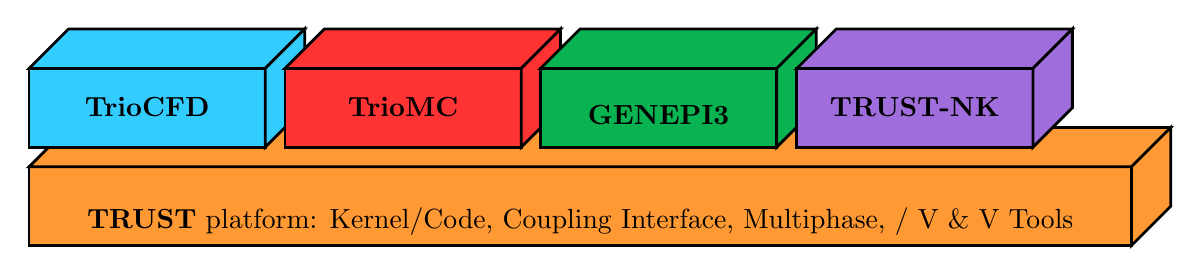
\begin{tikzpicture}[scale=2, line width=1pt]
% box TRUST
\coordinate (A) at (0,0) ;
\coordinate (B) at (7,0) ;
\coordinate (C) at (7,0.5) ;
\coordinate (D) at (0,0.5) ;
\coordinate (E) at (0.25,0.75) ;
\coordinate (F) at (7.25,0.75) ;
\coordinate (G) at (7.25,0.25) ;
\draw[black,fill=orange!80] (A) -- (B) -- (C) -- (D) -- cycle ;
\draw[black,fill=orange!80] (D) -- (C) -- (F) -- (E) -- cycle ;
\draw[black,fill=orange!80] (B) -- (C) -- (F) -- (G) -- cycle ;
\draw (3.5,0) node[above]{\textbf{TRUST} platform: Kernel/Code, Coupling Interface, Multiphase, / V \& V Tools} ;
%% box TrioCFD
\begin{scope}
\coordinate (A1) at (0,0.625) ;
\coordinate (B1) at (1.5,0.625) ;
\coordinate (C1) at (1.5,1.125) ;
\coordinate (D1) at (0,1.125) ;
\coordinate (E1) at (0.25,1.375) ;
\coordinate (F1) at (1.75,1.375) ;
\coordinate (G1) at (1.75,0.875) ;
\draw[black,fill=DeepSkyBlue!80] (A1) -- (B1) -- (C1) -- (D1) -- cycle ;
\draw[black,fill=DeepSkyBlue!80] (D1) -- (C1) -- (F1) -- (E1) -- cycle ;
\draw[black,fill=DeepSkyBlue!80] (B1) -- (C1) -- (F1) -- (G1) -- cycle ;
\draw (0.75,0.75) node[above]{\textbf{TrioCFD}} ;
\end{scope}
% box TrioMC
\begin{scope}[xshift=1.625 cm]
\coordinate (A1) at (0,0.625) ;
\coordinate (B1) at (1.5,0.625) ;
\coordinate (C1) at (1.5,1.125) ;
\coordinate (D1) at (0,1.125) ;
\coordinate (E1) at (0.25,1.375) ;
\coordinate (F1) at (1.75,1.375) ;
\coordinate (G1) at (1.75,0.875) ;
\draw[black,fill=red!80] (A1) -- (B1) -- (C1) -- (D1) -- cycle ;
\draw[black,fill=red!80] (D1) -- (C1) -- (F1) -- (E1) -- cycle ;
\draw[black,fill=red!80] (B1) -- (C1) -- (F1) -- (G1) -- cycle ;
\draw (0.75,0.75) node[above]{\textbf{TrioMC}} ;
\end{scope}
% box GENEPI3
\begin{scope}[xshift=3.248 cm]
\coordinate (A1) at (0,0.625) ;
\coordinate (B1) at (1.5,0.625) ;
\coordinate (C1) at (1.5,1.125) ;
\coordinate (D1) at (0,1.125) ;
\coordinate (E1) at (0.25,1.375) ;
\coordinate (F1) at (1.75,1.375) ;
\coordinate (G1) at (1.75,0.875) ;
\draw[black,fill=vert] (A1) -- (B1) -- (C1) -- (D1) -- cycle ;
\draw[black,fill=vert] (D1) -- (C1) -- (F1) -- (E1) -- cycle ;
\draw[black,fill=vert] (B1) -- (C1) -- (F1) -- (G1) -- cycle ;
\draw (0.75,0.7) node[above]{\textbf{GENEPI3}} ;
\end{scope}
%% box MPCube
\begin{scope}[xshift=4.875 cm]
\coordinate (A1) at (0,0.625) ;
\coordinate (B1) at (1.5,0.625) ;
\coordinate (C1) at (1.5,1.125) ;
\coordinate (D1) at (0,1.125) ;
\coordinate (E1) at (0.25,1.375) ;
\coordinate (F1) at (1.75,1.375) ;
\coordinate (G1) at (1.75,0.875) ;
\draw[black,fill=mauve!80] (A1) -- (B1) -- (C1) -- (D1) -- cycle ;
\draw[black,fill=mauve!80] (D1) -- (C1) -- (F1) -- (E1) -- cycle ;
\draw[black,fill=mauve!80] (B1) -- (C1) -- (F1) -- (G1) -- cycle ;
\draw (0.75,0.75) node[above]{\textbf{TRUST-NK}} ;
\end{scope}
\end{tikzpicture}
\caption{TRUST platform \& its BALTIKs}
\label{TRUST}
\end{center}
\end{figure}

\end{document}